\begin{mdframed}[style=warning]
	\begin{ejercicio}
		\textbf{Conceptos: }
		\begin{enumerate}[a)]
			\item Demuestre que la fuerza magnética no realiza trabajo.
			\item Considere un electrón en un campo eléctrico y magnético perpendiculares.
			\begin{itemize}
				\item ¿Qué trayectoria describe?
				\item ¿Cómo cambia dicha trayectoria si lo que viaja es un protón?
				\item ¿Qué pasa si la molécula es neutra?
			\end{itemize}
		\end{enumerate}
	\end{ejercicio}
\end{mdframed}











\begin{mdframed}[style=warning]
	\begin{ejercicio}
		Sabiendo que el momento dipolar magnético de una espira está dado por
		$$ \vec{\mu} = \frac{1}{2} \varointclockwise _{\Gamma} \qty(\vec{r} \cp I\dd{\vec{r}}), $$
		donde $\Gamma$ es la espira. Encuentre el momento dipolar magnético de una espira triangular con lados $L$, $L$ y $\sqrt{2} L$ y de una espira circular de radio $a$. Compare estos resultados con los obtenidos de la ecuación $\abs{\vec{\mu}} = IA$ con dirección dada por la regla de la mano derecha. \\
		\textit{Hint: El sentido de integración está dado por la corriente. Divida la espira en segmentos.}
	\end{ejercicio}
\end{mdframed}



















\begin{mdframed}[style=warning]
	\begin{ejercicio}
		Un disco metálico, de masa $m$ y radio $a$, se encuentra situado en una región en la que existe un campo magnético uniforme, $\vec{B}$, dirigido según su eje. Si el disco se pone a girar con velocidad angular $\vec{\omega}$, se establece una diferencia de potencial, $\Delta V$, entre el borde del disco y su eje de rotación.
		\begin{enumerate}[a)]
			\item Determine la fuerza magnética sobre las cargas libres del metal.
			\item Cuando se alcanza el estado estacionario, la resultante de las fuerzas eléctrica y magnética sobre las cargas libres del metal es nula. Si la velocidad angular $\vec{\omega}$ y el campo magnético tienen el mismo sentido, demuestre que la diferencia de potencial es
				$$ \Delta V = \frac{\Phi _B}{T}, $$
			donde $\Phi _B$ es el flujo de campo magnético y $T$ el periodo de rotación.
			\item Imagine que se conecta una resistencia exterior, $R$,  entre el eje y el borde del disco, de forma que permita el paso de corriente. La diferencia de potencial es la misma que existiría con el circuito abierto para esa velocidad angular. Llevando a cabo un balance de energía, demuestre que la energía cinética de rotación del disco, $E_c$, disminuye con el tiempo, por efecto Joule, de acuerdo con
				$$ \dv{E_c}{t} = -\frac{E_c}{\tau}, $$
			donde $\tau$ es un tiempo característico (con una idea parecida al de la constante de tiempo en un circuito $RC$). Exprese $\tau$ en términos de los parámetros conocidos.
		\end{enumerate}
		\begin{figure}[H]
			\centering
			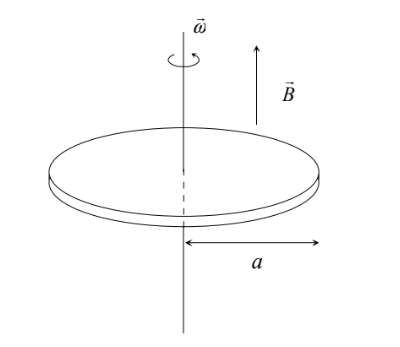
\includegraphics[scale=0.5]{./img/discoFaraday.png}
			\caption{Disco de Faraday.}
			\label{DF}	
		\end{figure}
	\end{ejercicio}
\end{mdframed}




















%%%%%


















































%%%